\documentclass{book}
\usepackage{pythonhighlight}
\usepackage{graphicx}
\usepackage{ctex}
\usepackage[left=3cm,top=3cm,right=3cm]{geometry}
\usepackage{hyperref}
\usepackage{amsmath}

%%%%%%%%%%%%%%%%%%%%%%%%%%%%%%
%writing instruction
%%%%%%%%%%%%%%%%%%%%%%%%%%%%%%

%插入代码
%\begin{python}
%..... 可以用 #。。。 写在行后表示注释
%\end{python}

%插入图片
%\begin{figure}[htbp]
%\centering
%\includegraphics[width=13.5cm]{img/....png}
%\caption{______fill in here____} %图片下方文字标签
%\label{img:zlt_pict1}   % 引用标记,用于文章中引用
%\end{figure}

%在文章中引用图片
%。。。,如图\ref{img:zlt_pict1}所示,。。。


\begin{document}

\title{EE208 Final Project Report \\ Integrated Search Engine for Elctronic Products \\ 电子商品集成搜索引擎}

\author{董世文 \quad 方少恒 \quad  杨弘博 \quad  周李韬 \\ GROUP 14 \\ SJTU F1803016} %%作者

\maketitle 

\tableofcontents 

\mainmatter %%表示文章的正文部分,在生成目录后将从第一页开始


\frontmatter

\chapter{前言}

本项目是本组同学经过一学期电类工程导论的学习,将网络爬虫、信息提取、索引查询、图像特征提取等知识和技能的整合和应用到一起,通过大作业的方式呈现的学习成果,实现了一个集成的电子产品商品搜索引擎。本项目的特色如下:
\begin{kaishu}
\begin{itemize}
\item 包含了3984条来源于苏宁易购的电子产品和6960条来源于京东的电子产品条目信息
\item 支持关键词检索、多字段检索
\item 支持图片匹配,提供LOGO识别和精确匹配两种模式
\item 支持对检索结果的价格、评分排序
\item 支持对检索结果的品牌、类别、特征、来源进行过滤
\item 提供基于商品评论数、评论标签的评分机制
\item 在搜索引擎中提供商品的部分具体信息
\end{itemize}
\end{kaishu}

在本项目的开发过程中,我们利用到了以下工具、框架和平台
\begin{kaishu}
\begin{itemize}
\item 基于Lucene搭建的索引和搜索引擎
\item 基于Web.py运行的前端框架
\item 基于Bootstrap的前端排版和美化
\item 基于Pyside.QtWebKit的网页提取工具
\end{itemize}
\end{kaishu}

本文将介绍本项目中主要功能的实现、效果和分析,本项目的源代码可以在GitHub\footnote{https://github.com/ltzone/EE208Lab}中获取。

\mainmatter


%%%%%%%%%%%%%%%%%%%%%%%%%%%%%%%%%%%
%%%%%%%PART I CRAWLER%%%%%%%%%%%%%%
%%%%%%%%%%%%%%%%%%%%%%%%%%%%%%%%%%%
\part{Crawler}

\chapter{京东爬虫}
\section{网页URL爬取}

制作一个商品检索网站,第一步要收集足量的商品信息。我们计划从京东和苏宁两家电商上爬取足量的数码类商品,来完成本次大作业。经过信息的分析整理,进行分类,打分,贴标签等信息的提取和完善,完成一个可用的,好用的商品检索网站。

由于大作业是小组协作,先爬取1w+的商品,得到一个记录商品url的index.txt,后面的一切工作都围绕这些商品展开。这个爬虫主要沿用的是第三次上机中完成的带banlist的多线程爬虫。以爬取京东的爬虫为例,相对早期代码,主要的改变主要是限制了爬取范围在形如“https://item.jd.com/\{\}.html.format(productID)”的url——我们只需要商品详情页的信息。体现在代码中就是改变了获取链接的格式:

\begin{python}
def get_all_links(content):
    if content == None:
        return []
    import re
    urlset = set()
    urls = re.findall(r"item.jd.com/[\^\\s]*.html",content,re.I)
    for u in urls:
        urlset.add('http://'+u)
    links = list(urlset)
    return links

\end{python}

此外,爬取的起点也要是商品详情页。

完成了爬取之后,我们还需要进行细节信息的提取,评论信息的提取和打分,以完成整个信息准备的工作。下面我们将对这些环节进行详细介绍。



\section{商品信息提取}
在爬取了一系列京东商品网址之后,我们获得了储存着这些网页URL和处理之后的文件名的文本。

接下来,为获取每件商品的详细信息,我们逐行读取该文本,通过打开每件商品网页的网址,结合beautifulsoup从content内容中截取我们需要的部分,并将其写入用来储存每件商品的具体信息的文本中。注意到京东旗下绝大部分商品网页的html布局都是相似的,我们可以通过定位固定的tag节点,并用“id”、“class”等属性加以限制,从而获取每一个商品网页中同一种商品信息的位置,完成爬取。

例如:我们观察到所有描述商品的图片地址在html中都保存在如图\ref{img:dsw1}所示的“img”标签下的“data-origin”类中,因此我们可以根据这一特点定位图片url的储存位置,利用find\_all()、get()等语句获取信息,并以读写方式将其写入文本文件中。

\begin{figure}[htbp]
\centering
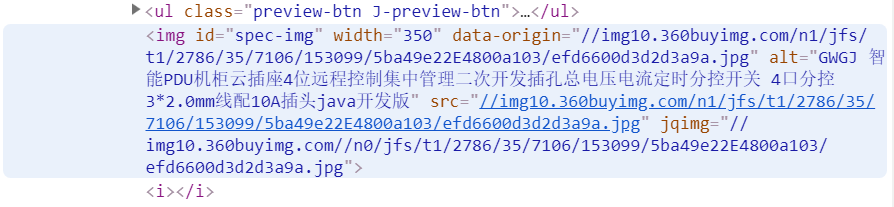
\includegraphics[width=13.5cm]{img/dsw/dsw1.png}
\caption{图片地址的获取}
\label{img:dsw1}
\end{figure}

获取imgurl的代码如下:
\begin{python}
    soup = BeautifulSoup(content,features='html.parser')
    for img in soup.find_all('img', id="spec-img"):
        src = img.get('data-origin', '')
        if (src == '' or not (src.endswith('jpg') or src.endswith('png'))):
            continue
        src = 'http:' + src
        with open(url + '.txt', 'a') as f3:
            f3.write(src)
            print src
            f3.write('\n')
\end{python}

其余商品属性的获取与之类似,比如在“class”为“parameter2 p-parameter-list”的“ul”标签下读取如图\ref{img:dsw2}所示的文本内容,我们可以获得如图\ref{img:dsw3}所示的商品属性:

\begin{figure}[htbp]
\centering
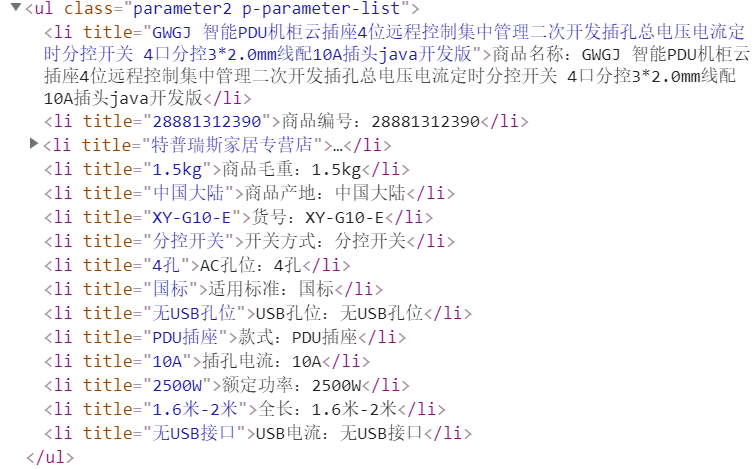
\includegraphics[width=10.5cm]{img/dsw/dsw2.png}
\caption{部分商品信息的获取}
\label{img:dsw2}
\end{figure}

\begin{figure}[htbp]
\centering
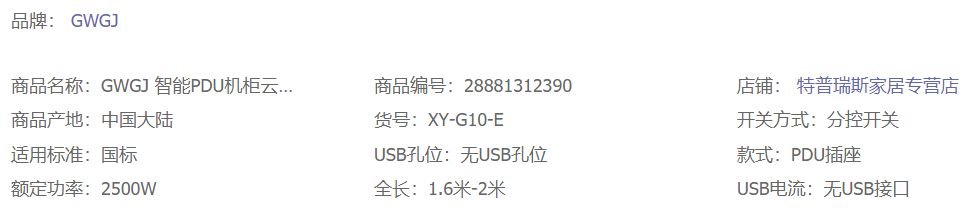
\includegraphics[width=13.5cm]{img/dsw/dsw3.png}
\caption{部分商品信息}
\label{img:dsw3}
\end{figure}

对这部分content进行字符串相关处理操作,就可以得到各项信息,并逐行写入文本中。

需要注意的一项商品属性是商品的价格。如果直接从content中读取价格对应标签下的内容,最终获得的价格就全部为空了。这是由于京东对价格进行了特殊的处理,我们不能像获取其他信息那样直接得到商品价格。在此我通过json获取mgets请求,从而得到了价格。请求语句如下,只保留skuIds这一项参数,其意为商品编号,而该编号可以从content中正常抓取。

\begin{python}
url2 = 'https://p.3.cn/prices/mgets?skuIds=J_' + str(k.contents[3].get('title'))
\end{python}

通过改变代码中的商品编号,我们可以得到类似于图\ref{img:dsw4}的响应,其中“p”对应的即为商品价格。(若当前商品已经下架,则“p” 值为-1)因此我们只需要获取该页面的文本,并定位到“p”字符后的数字即为价格。

\begin{figure}[htbp]
\centering
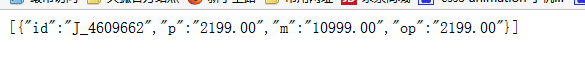
\includegraphics[width=11.5cm]{img/dsw/dsw4.png}
\caption{京东商品价格的获取}
\label{img:dsw4}
\end{figure}

当一件商品的相关detail全部被获取并储存之后,得到的文本如图\ref{img:dsw5}所示:共八行信息,从上到下依次为商品概述、网页URL、图片URL、商品名、品牌、价格、商品类别、其他属性。

\begin{figure}[htbp]
\centering
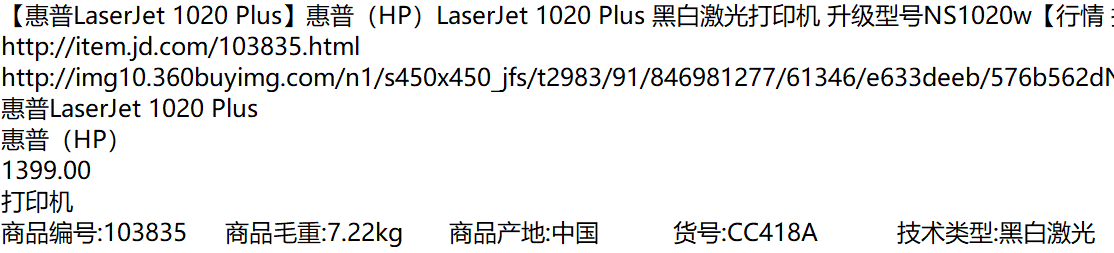
\includegraphics[width=12.5cm]{img/dsw/dsw5.png}
\caption{京东商品detail的保存}
\label{img:dsw5}
\end{figure}

至此,获取商品detail的部分就实现了。以上过程的实现代码保存在getdetail.py文件中。
\section{商品评论标签提取}
在了解了商品细节信息(如参数)之后,消费者通常也希望看到已买的人的评价,来作为自己是否要购买该商品的一个重要参考。于是乎,我们为了呈现这一部分信息,需要找到买家评价。但是,如图\ref{img:yhb1}所示,评价部分并不是直接显示在网页源代码中的。

%插入图片
\begin{figure}[htbp]
\centering
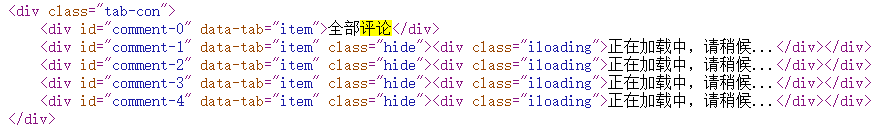
\includegraphics[width=13.5cm]{img/yhb/web_source_code_jd.png}
\caption{京东网页源码中查询评价的结果} %图片下方文字标签
\label{img:yhb1}   % 引用标记,用于文章中引用
\end{figure}

这也就是说,我们在之前爬到的HTML文件中是找不到评论信息的。
那么评论到底在哪里呢?简单想想,既然不在这个网址上,那么就一定在它会发送请求的某个网址上。下面不妨试一下,打开一个感兴趣的京东商品。我们在页面中鼠标右键选择检查(或F12)调出浏览器的调试窗口。然后点击network查看所有类型的请求(ALL),点击评论按钮使其加载数据。如图\ref{img:yhb2}所示。

%插入图片
\begin{figure}[htbp]
\centering
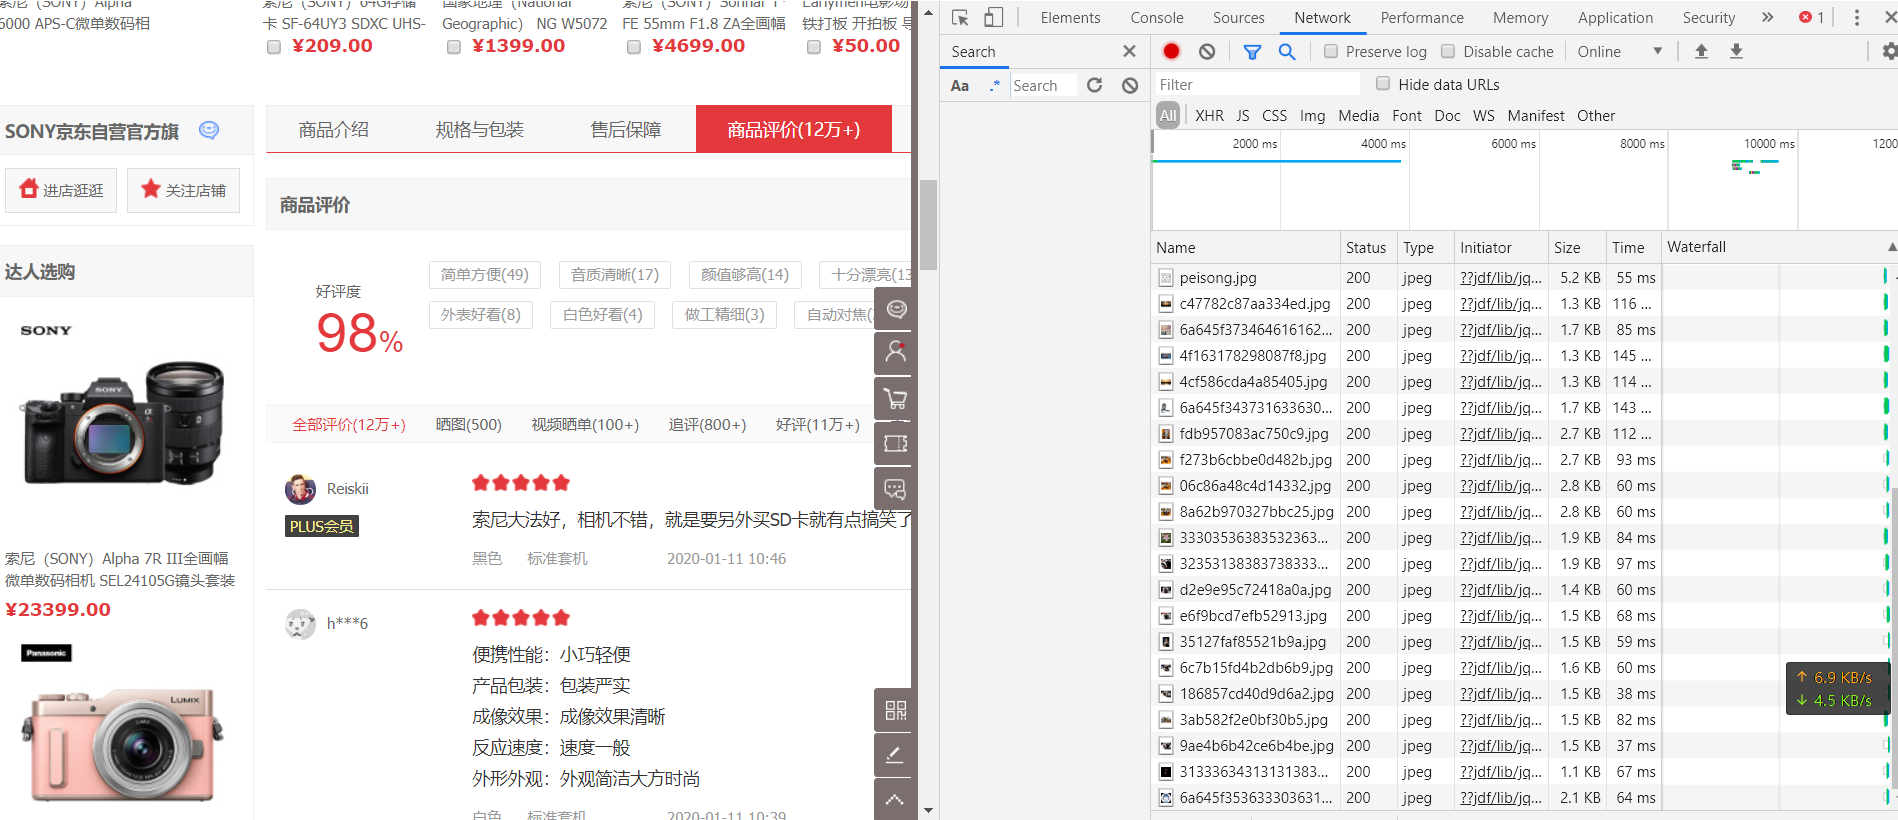
\includegraphics[width=13.5cm]{img/yhb/network_jd.png}
\caption{加载请求} %图片下方文字标签
\label{img:yhb2}   % 引用标记,用于文章中引用
\end{figure}

接着,查找加载评论数据的请求。我们可以使用某条评论中的一段话,然后在调试窗口中搜索。如图\ref{img:yhb3}所示。
%插入图片
\begin{figure}[htbp]
\centering
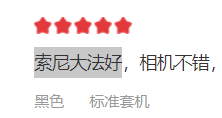
\includegraphics[width=3.5cm]{img/yhb/find_request_jd.png}
\caption{找到评论所在的请求} %图片下方文字标签
\label{img:yhb3}   % 引用标记,用于文章中引用
\end{figure}

搜索框下面返回的结果就是了。点击,在右面的headers里面可以看到request url,在preview里可以看到这个url里面的信息。如图\ref{img:yhb4}。
%插入图片
\begin{figure}[htbp]
\centering
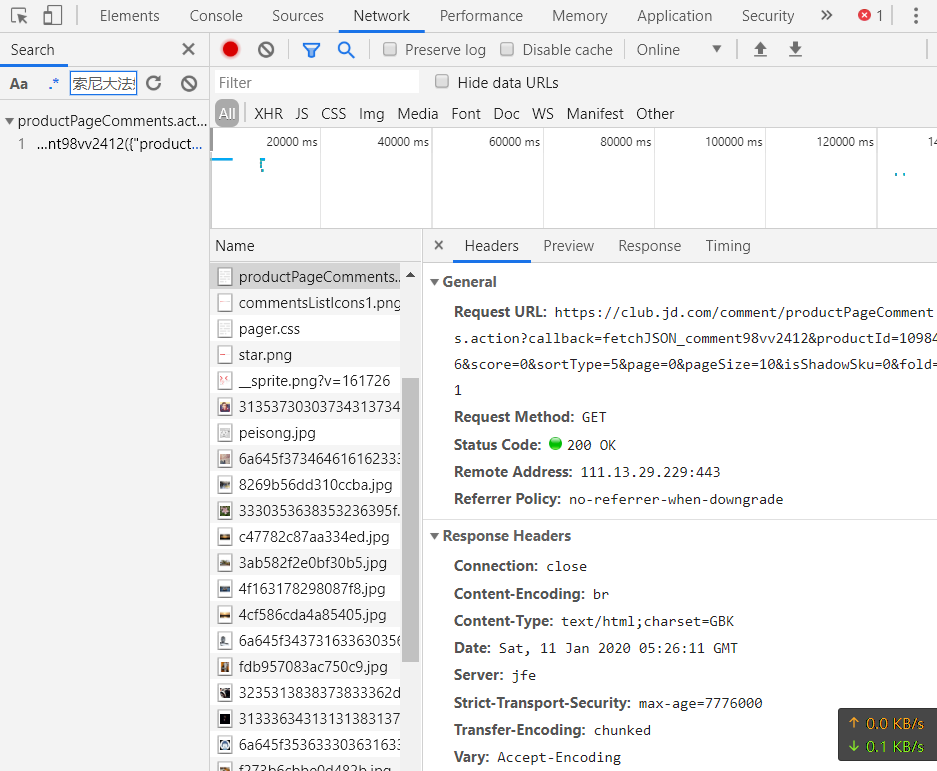
\includegraphics[width=10.5cm]{img/yhb/find_url_jd.png}
\caption{找到url} %图片下方文字标签
\label{img:yhb4}   % 引用标记,用于文章中引用
\end{figure}

在这个“fetchJSON\_comment”里面,有我们想要的评论信息。第一个标签comments,是评论的内容;第二个是评论的标签;第三个是评论的好评数量等数据统计。如图\ref{img:yhb5}所示。

%插入图片
\begin{figure}[htbp]
\centering
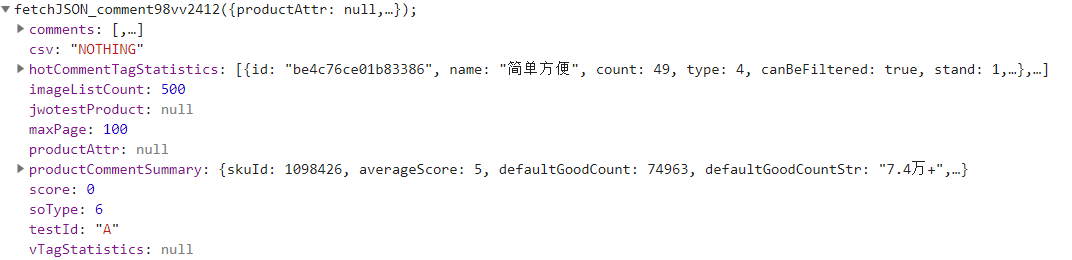
\includegraphics[width=13.5cm]{img/yhb/json_items_jd.png}
\caption{京东评论请求内容}
\label{img:yhb5}   % 引用标记,用于文章中引用
\end{figure}



一开始完成这个脚本的时候,设计的功能是将评论的内容(第一部分)爬下来。图\ref{img:yhb6}展示了一些例子。
\begin{figure}[htbp]
\centering
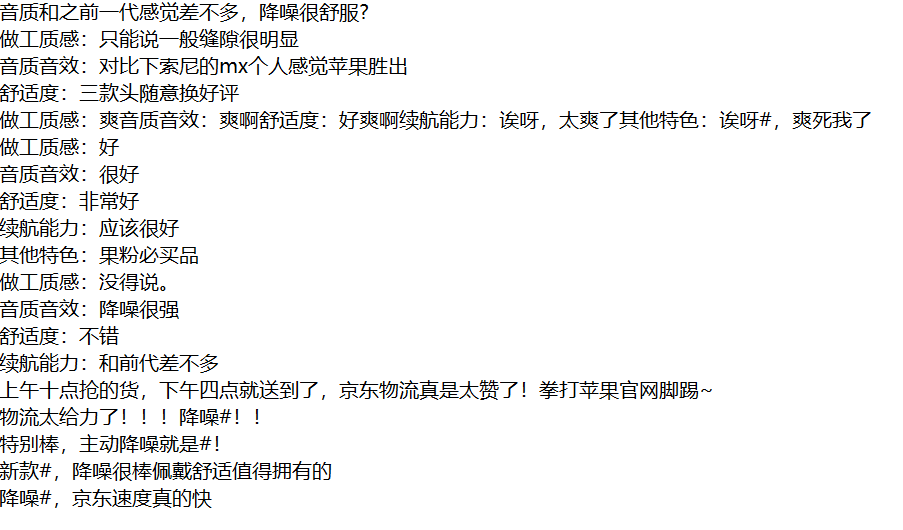
\includegraphics[width=9.5cm]{img/yhb/cmt_contents_eg_jd.png}
\caption{airpods pro的评论文字} %图片下方文字标签
\label{img:yhb6}   % 引用标记,用于文章中引用
\end{figure}

但这样做存在问题:一是,对于我一开始爬的上万个商品,将评论的文字全部弄下来空间占用太大了,建索引也会不方便;二是,我们想要实现的是商品的聚类检索,点击商品标签是可以直接跳到原商品网页的,不能,也没有必要在搜索结果上显示评论。因此,我希望通过商品的\textbf{评论标签}来对商品的特性进行说明。并通过\textbf{打分}来给商品一个基本的评定。

在明确了任务,并找到了接口之后,我们就可以开始写代码抓取数据了。一般我们会先尝试抓取一条数据,成功之后,我们再去分析如何实现大量抓取。下面的代码是在Windows环境下的python3里实现的。

\subsection{爬取评论数据}
经过上面的寻找和分析,可以确定url具有下面的格式:
%插入代码
\begin{python}
url=r"https://sclub.jd.com/comment/" \
    r"productPageComments.action?callback=fetchJSON_comment98vv106813&" \
    r"productId={}&" \
    r"score=0&sortType=5&page=0&pageSize=10&isShadowSku=0&fold=1".format(prdtId)
comment_tag_path = r'C:\TC-prog\JetBrain_pycharm_TC' \
                   r'\PycharmProjects\Crawler_EEFinal' \
                   r'\jd_cmt_tags\httpsitem.jd.com{}.html.txt'.format(prdtId)
try:
    r=requests.get(url,headers=headers,timeout=5)
    r.raise_for_status()
except:
    print ('爬取失败')
\end{python}
通常,我们会对爬虫脚本进行伪装,使之看起来更像是浏览器。下面设置请求中头文件的信息:
%插入代码
\begin{python}
headers = {'User-Agent':'Mozilla/5.0 '
                        '(Windows NT 10.0; Win64; x64) '
                        'AppleWebKit/537.36 (KHTML,'
                        ' like Gecko) Chrome/76.0.3809.132 '
                        'Safari/537.36',
                        'Referer':'https://www.jd.com/'
}
\end{python}
如果没有这个请求头,request返回的内容很有可能为空。

\subsection{提取数据}
我们对爬取的数据分析发现,此数据为跨域请求返回的json结果,所以我们只要把前面的“\textbf{fetchJSON \_ comment98vv4646(}”和最后的“\textbf{)}”去掉就拿到json数据了。

\begin{python}
raw = r.text[:]
pos = 0#这样写可以裁掉不一样长的前面这一串
for i in range(len(raw)):
    if raw[i] == '(':
        pos = i
try:
    r_json_str = r.text[pos + 1:-2]
    # print (r_json_str)
    r_json_obj=json.loads(r_json_str,strict=False)
    print (r_json_obj)
    r_json_tags=r_json_obj['hotCommentTagStatistics']
    print ('评论标签:')
\end{python}
上面的代码需要调用json库,json.loads函数将json对象转化成python的内置类型,在这里是字典。后面就按python dict类型进行操作了。

由图\ref{img:yhb7}可见,每一个标签名都是在name字段下的,对应的数目是count。

%插入图片
\begin{figure}[htbp]
\centering
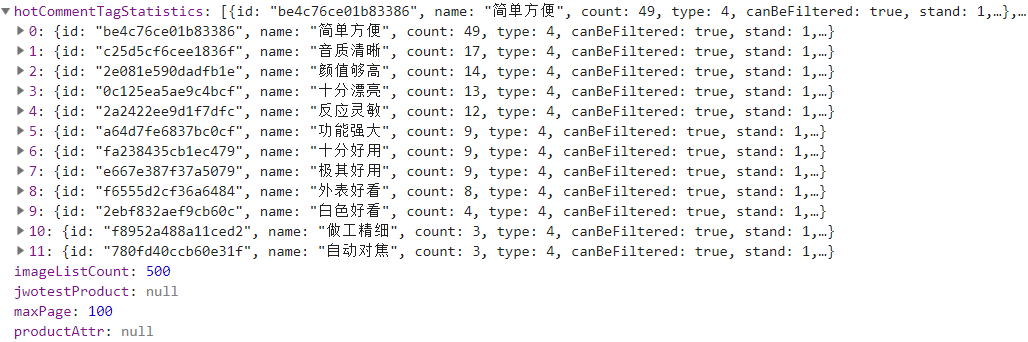
\includegraphics[width=13.5cm]{img/yhb/cmt_tags_eg_jd.png}
\caption{评论标签请求内容}
\label{img:yhb7}   % 引用标记,用于文章中引用
\end{figure}

可以根据这点读取评论的标签和数量:

\begin{python}
print(r_json_tag['name']+
                      '\t'+str(r_json_tag['count']))
\end{python}

\subsection{写入文件}

数据提取后我们需要将他们保存起来,一般保存数据的格式主要有:文件、数据库、内存这三大类。今天我们就将数据保存为txt文件格式,因为操作文件相对简单同时也能满足我们的后续数据分析的需求:

\begin{python}
# 追加模式,逐行写入
        for r_json_tag in r_json_tags:
            with open(comment_tag_path,'a+') as file:
                file.write(r_json_tag['name']+
                           '\t'+str(r_json_tag['count'])+'\n')
                print(r_json_tag['name']+
                      '\t'+str(r_json_tag['count']))
\end{python}

由于后面进行批量爬取的时候很有可能出现爬取失败的情况,上面的内容要放进try\&except里。

\subsection{批量爬取及多线程}

由于要处理的对象数目庞大,仅仅使用线性的程序不只是慢,而且可靠性也会大打折扣。所以这个脚本需要写成多线程的,来保证程序不会因为一个线程的终止而停下来。

注意到请求的url具有相对稳定的格式,仅有两处是变化的:一是“fetchJSON\_...”这样的一串,二是后面的商品ID(通过商品页url可以过滤出来)。经过多次实验,可以发现对于第一串,只要具有形如fetchJSON\_...的格式,请求往往都是可以被接受的。于是在封装的函数里,比较容易写出一般形式的url:

\begin{python}
url=r"https://sclub.jd.com/comment/" \
        r"productPageComments.action?callback=fetchJSON_comment98vv106813&" \
        r"productId={}&" \
        r"score=0&sortType=5&page=0&pageSize=10&isShadowSku=0&fold=1".format(prdtId)
\end{python}

将前面的步骤封装进函数后,设置多线程如下所示

\begin{python}
def crawl_jd_cmt_tag(prdtId):
    ...
q = queue.Queue()
NUM = 5
JOBS = 10
def run():
    global f
    for line in f.readlines():
        try:
            ... # 获取itemID
            crawl_jd_cmt_tag(itemID) # 运行爬取函数
            time.sleep(random.random() * 3)
        except:
            print("Invalid Input!")
def working():
    while True:
        run()
        q.task_done()
#fork NUM个线程等待队列
for i in range(NUM):
    t = Thread(target=working)
    t.setDaemon(True)
    t.start()
#把JOBS排入队列
for i in range(JOBS):
    q.put(i)
#阻塞,等待所有JOBS完成
q.join()
f.close()
\end{python}

有必要解释一下run函数中的工作。爬取2w+条商品生成了一个记录了这些商品的url的表格(.txt)。而这些url中含有对应每个商品的ID。run函数的工作就是抽出ID,调用专用于评论的爬虫函数,来记录评论标签。

运行结果如图\ref{img:yhb8}、\ref{img:yhb9}所示。下面,我们将按相似的流程完成商品的评分。

%插入图片
\begin{figure}[htbp]
\centering
\begin{minipage}[t]{0.48\textwidth}
\centering
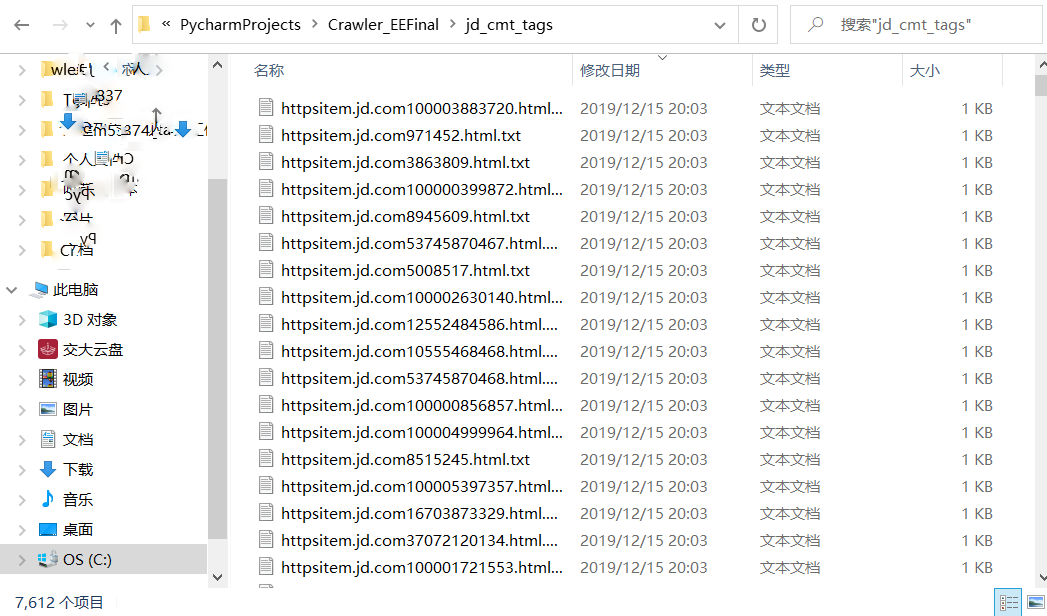
\includegraphics[height=5cm]{img/yhb/folder_view_jd.png}
\caption{爬取结果示例}
\label{img:yhb8}  
\end{minipage}
\begin{minipage}[t]{0.48\textwidth}
\centering
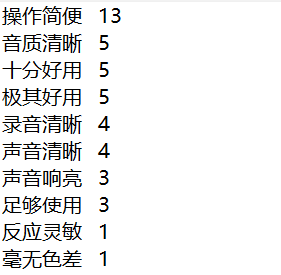
\includegraphics[height=4cm]{img/yhb/contents_eg_jd.png}
\caption{爬取结果示例}
\label{img:yhb9}  
\end{minipage}
\end{figure}   % 引用标记,用于文章中引用


\section{商品评分计算}
程序的工作流程和整体框架和爬取标签时的一样,但需要更改存储路径和对json对象信息的处理方式。具体来说,需要抽取不同属性的数据,并设计一个评估商品优劣的数值算法。preview该请求,看一下productCommentSummary里的内容,如图\ref{img:yhb10}所示。

\begin{figure}[htbp]
\centering
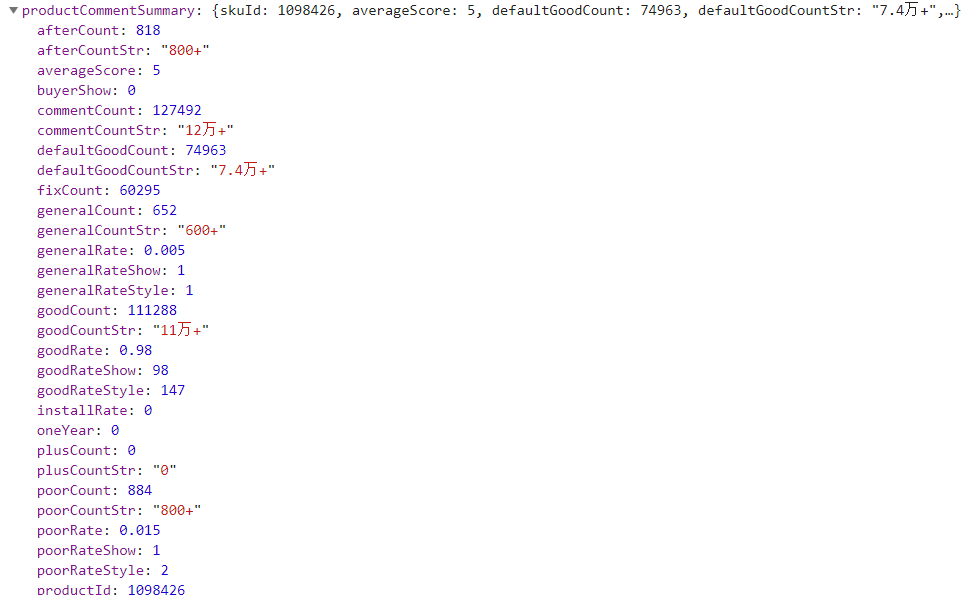
\includegraphics[width=8.5cm]{img/yhb/data_eg_jd.png}
\caption{productCommentSummary内容的部分截图}
\label{img:yhb10}  % 引用标记,用于文章中引用
\end{figure}

在这些数据里,好评率可以反映消费者的满意程度,评论总数可以反映商品销量和热度,追评和视频评价则可以一定程度体现消费者对商品的重视程度。将这些信息综合考虑,可以设计下面计算商品分数的公式:

\begin{python}
score=int(rate*0.7+math.log10(sumcmt)*5+
                          ((after+video)*1.0)/sumcmt/0.05)
\end{python}

实现打分的代码块如下:
\begin{python}
    try:
        r_json_str = r.text[pos + 1:-2]
        r_json_obj=json.loads(r_json_str,strict=False)
        r_json_Sum=r_json_obj['productCommentSummary']
        with open(comment_tag_path, 'w') as file:
            sumcmt=r_json_Sum['commentCount']
            rate=r_json_Sum['goodRateShow'] # 好评率*100
            video =r_json_Sum['videoCount']
            after =r_json_Sum['afterCount']
            score=int(rate*0.7+math.log10(sumcmt)*5+
                          ((after+video)*1.0)/sumcmt/0.05)
            file.write("httpitem.jd.com"+str(prdtId) +".html"
                       + '\t' + str(score) + '\n')
            print("httpsitem.jd.com"+str(prdtId) +".html"
                       + '\t' + str(score))
    except:
        print('failed')
\end{python}

运行结果如图\ref{img:yhb11}、\ref{img:yhb12}所示。



%插入图片
\begin{figure}[htbp]
\centering
\begin{minipage}[t]{0.48\textwidth}
\centering
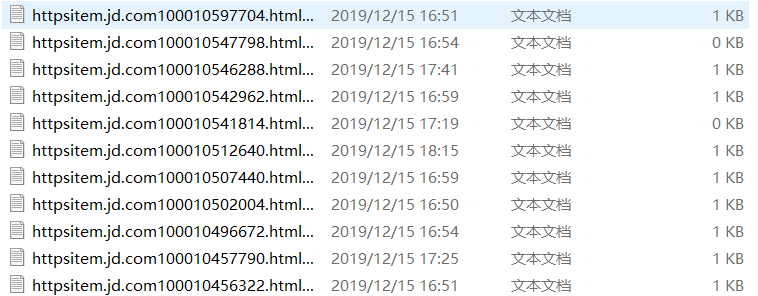
\includegraphics[width=5cm]{img/yhb/res1_jd.png}
\caption{评论打分内容示例}
\label{img:yhb11}
\end{minipage}
\begin{minipage}[t]{0.48\textwidth}
\centering
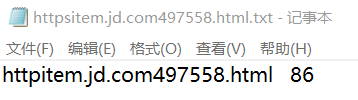
\includegraphics[width=4cm]{img/yhb/res2_jd.png}
\caption{评论打分内容示例}
\label{img:yhb12} 
\end{minipage}
\end{figure}   % 引用标记,用于文章中引用


到这里,我们就完成了京东的评论标签爬取和分数评定。后面对苏宁爬取商品也将采取类似的这些操作。



\chapter{苏宁爬虫}
\section{商品信息爬取}
fsh
\section{商品评论标签爬取}
yhb
\section{商品评分计算}
yhb



%%%%%%%%%%%%%%%%%%%%%%%%%%%%%%%%%%%
%%%%%%%PART II INDEXER%%%%%%%%%%%%%
%%%%%%%%%%%%%%%%%%%%%%%%%%%%%%%%%%%


\part{Index \& Search}
\chapter{构建索引}
在获取了商品属性、用户评价、商品打分等内容并分别将其储存在文本文件中后,我们接下来就可以利用Lucene建立索引了。由于京东和苏宁的商品信息都是这三类并且以相同的格式存储,我们接下来以京东为例解释建立索引的过程。

与本学期第五次试验建立Lucene索引的过程类似,首先我们打开一个储存有所有商品网址和文件名的文本,逐行读取商品URL和文件名,并从detail、 comment、score三个文件夹中找到储存该网页对应信息的三个文本。分别打开这三个文本文件,读取其中内容并进行合适的格式处理,最终添加为field。

我们的fieldType配置如下表所示。
\begin{table}[h]
\begin{tabular}{lccc}
\hline
\multicolumn{1}{c}{\textbf{FieldName}} & \textbf{Indexed} & \textbf{Stored} & \textbf{Tokenized} \\ \hline
URL                                    & T                & T               & F                  \\
price 商品价格                             & \multicolumn{3}{c}{built-in LONG Type}                  \\
score 商品评分                             & \multicolumn{3}{c}{built-in LONG Type}                  \\
imgurl 商品图片地址                          & F                & T               & F                  \\
title 商品名称                             & T                & T               & T                  \\
brand 商品品牌                             & T                & T               & T                  \\
attribute 商品类别                         & T                & T               & F                  \\
detail 商品详情                            & F                & T               & F                  \\
tag 商品标签                               & F                & T               & F                  \\
website 商品来源                           & F                & T               & F                  \\ \hline
\end{tabular}
\end{table}


首先注意到,价格“price”和打分“score”。前者从保存“detail”的文本中获取,后者则专门保存在“score”的文本中。由于这两样内容需要进行后续的数值比较,我们不能将其与其他field一样以“str” 形式建立,而要将之转换为long的格式,并建立longfield。以“score”为例:

\begin{python}
path3="new/score/" + filename2 + ".txt"
ff3 = open(path3)
line = ff3.readline().strip()
score = int(line.split('\t')[1])        #截取score
scoree = long(score)                    #转换为long型数
doc.add(LongField('score', scoree, Field.Store.YES)) #建立longfield,设为可存储
\end{python}


其次,商品标题(即商品简述)“title”。为了后续的检索,我们这里需要利用SimpleAnalyzer以及jieba分词库对其进行分词处理,并允许indexed、stored、tokenized。

此外,商品品牌、商品类别,由于是每个商品共有的属性,而且在多字段查询中也会被检索,因此我们也进行了索引或分词。

苏宁商品信息的索引建立过程与京东类似。至此,Lucene索引就建立完毕了。具体代码见文件“makeindex.py”。


\chapter{图片匹配}

\section{LOGO匹配}

在商标识别中,我们实现的功能为用户上传一张图片,返回最匹配的商标的名称。我们建立了一个商标的图片库(logo\_recognition/logo\_images)以及一个商标索引(brands.txt),对每张上传的图片,逐一与图片库中的图片比较sift特征向量,每个品牌的得分为该品牌下每张图片与待测图片的匹配特征点个数的平均值,最后返回得分最高的品牌。

特征点的选择以及特征向量的计算使用opencv库中的SIFT\_create.detectAndCompute函数。

\begin{python}
detector = cv2.xfeatures2d.SIFT_create() # 特征向量计算使用sift算法
QueryImgBGR=cv2.imread(img)
QueryImg=cv2.cvtColor(QueryImgBGR,cv2.COLOR_BGR2GRAY) # 读取图片灰度图
QueryImg = cv2.GaussianBlur(QueryImg, (3, 3), 0) # 高斯模糊,降点噪点影响
queryKP,queryDesc=detector.detectAndCompute(QueryImg,None) # queryKP,queryDesc为特征点坐标以及特征向量的列表
\end{python}

我们使用FlannBasedMatcher寻找最近邻近似匹配,使用knnmatch匹配处理,返回匹配的特征点对,当两特征值的欧式距离小于一定值时视为匹配成功。

\begin{python}
scores = []
flannParam = dict(algorithm = 0,tree = 5)
flann = cv2.FlannBasedMatcher(flannParam,{}) # 最近邻近似匹配

for brand in brands:
    trainImg = []
    score = 0.0
    for filename in glob.glob('logo_images/%s/*' %brand): # 遍历单个品牌图片库中的所有图片,读取图片信息
        im = cv2.imread(filename,0)
        im = cv2.GaussianBlur(im, (3,3), 0)
        trainImg.append(im)
    for num in range(len(trainImg)):
        trainKP,trainDesc=detector.detectAndCompute(trainImg[num],None) # 获得品牌图片的特征点以及对应sift特征向量信息
        matches=flann.knnMatch(queryDesc,trainDesc,k=2) # 使用knnmatch匹配,k=2:返回2个DMatch数据类型
        goodMatch=[]
        for m,n in matches:
            if(m.distance<0.75*n.distance): # 计算两对特征值的欧氏距离大小差,此处阈值设为0.75
                goodMatch.append(m)
        score = score+ len(goodMatch)
    scores.append(score/len(trainImg)) # 每个品牌的得分为该品牌图片库特征点匹配个数的平均值

print(brands[scores.index(max(scores))]) # 返回得分最高的品牌
\end{python}

\section{图片搜索}

我们使用LSH(Locality-sensitive Hashing)算法实现商品的图片搜索。主要原理是先通过颜色直方图的方法提取图片库中所有图片的特征向量,转化为hamming code,用5个不同的哈希函数映射到5张哈希表中,将哈希表保存在外存中。在图片搜索的时候,对查询的图片用相同的哈希函数映射,返回哈希表中相同的bucket里的图片。

\subsection{图片特征向量提取}

图片特征向量通过颜色直方图的方式获得。先将图片划为8*8的64小格,由于图片皆为数码产品,图片四周有大量空白,我们在提取特征向量时只考虑图片中心的4*4小格。对16(4*4)小格分别计算颜色直方图,将颜色直方图中的R、G、B按一定比例划分映射到0到2的整数,因此每张图片可以得到一个48维的特征向量。

将颜色比例映射到整数的划分为0-0.31到0,0.31-0.355到1,0.355-1到2。由于数码产品的商品图大多接近纯黑或者纯白,RGB的比例分布大多接近0.333,为了让特征向量的值尽可能均匀的分布,我们选择的划分很接近三分之一,这样能尽可能凭借特征向量区分相似图片和不同图片。

\begin{python}
def get_feature(imgurl):
    # 通过图片url下载图片,以rgb格式读取图片
    img = "1.jpg"
    urllib.urlretrieve(imgurl,filename="1.jpg") # 将图片保存在本地的1.jpg中
    img=cv2.imread(img,cv2.IMREAD_COLOR)
    os.remove("1.jpg") # 删除1.jpg文件

    imginfo = img.shape # 计算每小格尺寸
    height = int(math.floor(imginfo[0]/8))
    width = int(math.floor(imginfo[1]/8))

    # 计算图片特征向量
    des = [] # 图片特征向量
    for p in range(2,6):
        for q in range(2,6):
            e_b = 0.0
            e_g = 0.0
            e_r = 0.0
            h_b = 0
            h_g = 0
            h_r = 0
            for i in range(height):
                for j in range(width):
                    b,g,r = img[i+p*height,j+q*width]
                    index_b = int(b)
                    index_g = int(g)
                    index_r = int(r)
                    if index_b+index_g+index_r:
                        e_b += float(index_b)/(index_b+index_g+index_r)
                        e_g += float(index_g)/(index_b+index_g+index_r)
                        e_r += float(index_r)/(index_b+index_g+index_r)
            if e_b+e_g+e_r: # 计算颜色直方图
                h_b = e_b/(e_b+e_g+e_r)
                h_g = e_g/(e_b+e_g+e_r)
                h_r = e_r/(e_b+e_g+e_r)
            for i in [h_b, h_g, h_r]: # 将R、G、B映射的整数加入图片特征向量中
                if i < 0.31:
                    des.append(0)
                elif i > 0.355:
                    des.append(2)
                else:
                    des.append(1)

    return des
\end{python}

\subsection{哈希函数映射}

哈希函数先将特征向量转换为二进制的hamming code,参数proj表示hamming code投影的位数,列表proj的长度即为二进制哈希值的长度。

\begin{python}
# 哈希函数定义
def LSHash(des,proj):
    C = 2
    length = len(des)
    projlength = len(proj)
    idx = 0
    hash_result = []
    for i in range(length):# 原向量的第i位
        i_proj = []
        while (proj[idx]<=(i+1)*C):
            i_proj.append(proj[idx]-i*C-1)
            idx += 1       # 获取第i位中需要的投影数
            if (idx >= projlength):
                break
        for i_proj_elem in i_proj:  # 计算第i位投影hamming code,加入哈希结果
            if des[i] > i_proj_elem:
                hash_result.append(1)
            else:
                hash_result.append(0)
        if (idx >= projlength):  # proj已经遍历完,退出
            break
    # hamming code转十进制
    sum = 0
    multi = 1
    for x in hash_result:
        sum += multi*x
        multi*=2
    return sum
\end{python}

我们选择五个哈希函数将图片的特征向量通过hamming code的转换映射到一个12位二进制数,转换为十进制即即0到4095,因此需要规模为4096的哈希表。哈希表以数组的结构保存,图片对应的网页以及图片的特征向量在哈希表中的保存位置即为十进制哈希值的大小。

\begin{python}
hash_table = [[[] for i in range(4096)] for j in range(5)] # 构建五个大小为4096的空哈希表
folder_1 = '../sn_crawler/html_sn' # folder_1为保存页面信息的文件夹
projs = [ \
    [7, 10, 16, 21, 23, 34, 45, 48, 61, 62, 69, 77], 
    [12, 20, 23, 30, 32, 40, 57, 61, 62, 70, 78, 94], 
    [10, 14, 18, 21, 25, 33, 39, 44, 50, 67, 91, 93], 
    [13, 18, 19, 42, 52, 65, 67, 68, 71, 88, 90, 92], 
    [4, 6, 15, 23, 28, 37, 45, 46, 62, 81, 83, 93]] # 哈希函数的proj参数

for root, dirs, files in os.walk(folder_1):
    for file in files:
        try:
            url,imgurl = getUrl(folder_1,file) # getUrl函数:从已爬取信息中提取图片的url地址以及对应商品的url地址
        except Error:
            print "Error"
            continue

        det = get_feature(imgurl)
        d = [url,det] # 哈希表中保存的内容为图片对应的商品页面url以及图片的特征向量
        for j in range(5):
            hash_val = LSHash(det,projs[j])
            hash_table[j][int(hash_val)].append(d)

# 将构建好的哈希表以json格式保存
with open("hash_table.json",'w') as file_obj:
    json.dump(hash_table,file_obj)
\end{python}

\chapter{商品检索与排序}

前文所述过程中建立的Lucene索引表和图像LSH哈希表是本章节商品检索与排序的根据,在本项目中,我们实现了两种检索方式——按关键词检索与按图片检索。

按关键词检索部分,用户可以输入商品关键词执行检索,也可以输入商品的品牌等属性执行高级检索。对检索的结果,用户可以选择按照相关度、价格顺序、评分高低进行排序。在图片检索中,用户上传图片后,可以选择LOGO匹配或精确匹配两种方式。LOGO匹配将图片与我们建立的产品品牌图库中的LOGO对比,计算SIFT特征向量的相似度,返回最有可能的品牌关键词执行关键词检索。精确匹配则将图片特征向量映射到前文建立的LSH哈希表中,返回匹配图片的URL列表,再到Lucene索引表中调用TermQuery匹配出URL对应的条目,按匹配度返回商品信息到前端中。关键词检索与相关度排序沿用了本课程此前实验的代码,不作详述。本章节将主要介绍高级检索、商品排序和图片匹配三个功能的实现。

\section{商品高级检索}


\subsection{接口设计}

在此前建立索引的过程中,对于所有商品都具备的属性,如品牌、来源网站等,我们建立了专门的可被索引的Field进行存储,在本节我们将实现对这些Field的多字段检索。

在编写检索程序的代码前,考虑到我们的项目需要整合多种检索和排序方式,包括关键词、多字段检索、价格排序、评分排序等,我们有必要做好统一的接口,实现多重功能在后端查询时的一致。

一方面,用户可能在高级查询页面给出多字段的查询请求,对此我们采取了此前实验中类似的方法,编写了一个commandParser将查询条件转换成BooleanQuery处理多字段查询的请求。尽管在查询首页中,用户输入的数据是以表单形式传入的,但我们在编写查询程序时仍旧先将其转换成了一条“contents site:... brand:...”的字符串形式。我们之所以不直接提取表单内容,是我们出于下文实现filter功能的考量,在filter功能中,用户在勾选过滤选项后会再次发出一个包含搜索的请求,网页需要保存记录此前搜索的字段传入filter请求的参数中,为了便于代码的复用,转换成字符串的方式会使程序更加可读和清晰。

另一方面,用户在结果页面可能会选择不同的检索方式,这会决定Lucene检索过程中searcher的参数,我们需要为此编写不同的搜索函数。在综合考虑整合以上两种因素后,以下是我们为检索程序提供的接口,可以看到,商品检索程序位于search\_command中,需要提供检索字符串kw和method(默认为按相关度relativity排序)两个参数。对获得的商品信息我们会做一些处理,获得filtertags等信息,具体将在前端部分进行介绍。

\begin{python}
# 统一处理搜索请求的web脚本 Web/code.py
class search:
    def GET(self):
        user_data = web.input(website="",brand="")
        kw = user_data.keyword
        if user_data.brand:
            kw += ' brand:%s' %(user_data.brand)
        if user_data.website:
            kw += ' website:%s' %(user_data.website)   # 将输入表单转换成字符串形式的请求
        method = web.input(method="relativity").method.decode('utf-8')
        vm_env.attachCurrentThread()
        contents = search_command(kw,method)     # 搜索结果
        filtertags = total(contents)           # 统计品牌、属性、特色的结果,即显示在页面左侧所必须的内容
        results = itemlis(contents)            # 要显示在页面右侧的所必需的内容
        return render.result(kw,method, results, filtertags)
\end{python}

\subsection{多字段查询处理}

在检索程序中,我们首先要对输入的query字符串进行处理,为此我们编写了一个command\_to\_query函数,统一处理各种形式的query。

\begin{python}
def command_to_query(command,analyzer):
    command_dict = parseCommand(command)          # 将字符串query转换成dict形式
    print command_dict
    seg_list = jieba.cut(command_dict['title'])
    command_dict['title'] = (" ".join(seg_list))  # 对command_dict遍历,建立BooleanQuery
    querys = BooleanQuery()
    for k,v in command_dict.iteritems():
        query = QueryParser(Version.LUCENE_CURRENT, k,
                            analyzer).parse(v)
        querys.add(query, BooleanClause.Occur.MUST)  # 各字段之间为AND关系
    return querys
\end{python}

对不同的检索方式,我们设计了如下结构以调用不同的搜索函数。
\begin{python}
def search_command(query,method):
    ... # 配置searcher、analyzer
    return globals()[method+'_search'](searcher,analyzer,query)
    # 根据method的不同调用不同函数名的搜索函数
\end{python}

至此,我们完成了搜索程序接口的设计,并且实现了商品的多字段高级搜索。

\section{商品按属性排序}

对具体的函数设计而言,我们有按相关度排序、按价格排序和按评分排序。相关度排序检测搜索结果与商品名称信息的匹配度,可以调用Lucene内置的scoreDocs方法实现,在此前的实验中已经完成,不作详述。对价格和评分排序,我们在建立索引时已经将这些信息用Lucene内置的LONG Field进行存储,我们只需为其建立对应的SortField,Lucene就可以实现按排序执行查找,以按评分查找为例,对应搜索程序的脚本如下所示。

\begin{python}
def rank_search(searcher, analyzer, command):
    rank_sorter = Sort(SortField("score",SortField.Type.LONG,True))  # True表明降序排序
    query = command_to_query(command,analyzer)
    scoreDocs = searcher.search(query, 150, rank_sorter).scoreDocs
    return read_results(scoreDocs,searcher) 
    # read_results函数提取搜索结果中的必要信息,将在前端部分介绍
\end{python}

\section{按图片检索}

\subsection{图片匹配}
根据我们已经建立的Hash表中包含了网页的URL和直方图特征向量。执行查询时,对输入的图片文件,我们计算图片文件的特征向量,将特征向量通过建表时相同的哈希函数映射到5张哈希表中,由LSH的局部敏感性质,我们认为哈希映射击中单元中的所有元素都和查询query具有一定的相似性。取5张哈希表中击中单元的并集,计算待查询的特征向量与我们存储的特征向量的相似度,就可以按序给出最接近的若干URL。

在查询的过程中,我们仅计算了5个哈希值,并仅对取出的n个元素(n远远小于数据集规模N)计算了匹配度,因此所消耗的时间是与数据集无关的常数时间。此外,由于我们的特征向量已经存放在了哈希表中,因此也可以保证计算匹配度的时间相较数据集规模N是常数的。该查询方式能够在时间上达到理想的效率。

\begin{python}
# 匹配图片函数
def match_pict(img):
    docs = []
    imgfeat = get_feature_Local(img)             # 计算查询图片的特征向量
    with open("hash_table.json",'r') as load_f:  # 打开本地哈希表文件
        load_list = json.load(load_f)
        for j in range(0,5):
            hash_val = LSHash(img,proj[j])       # 对查询图片进行哈希映射
            hits = load_list[int(hash_val)]      # 取出映射结果
            for hit in hits:
                elem = hit[0],similarity(imgfeat,hit[1])
                if elem not in hit:
                    hit.append(elem)             # 加入待排序集
    docs_sorted = sorted(docs,key = lambda kv:(kv[1]))
    res_lis = [i for (i,j) in docs_sorted[:50]]  # 取前50匹配的结果
    return res_lis                               # 返回50个最匹配的URL条目
\end{python}

\subsection{匹配条目查询}

上述过程中返回了一个URL列表,注意到URL是区分不同商品信息的标准,因此理论上有了URL就可以将搜索结果呈现在网页中。但不同于其他查询方式中返回包含所有信息的索引文档列表,在这里我们还需要对哈希表返回的URL列表元素在Lucene索引库中再查询,以获得商品的完整信息呈现在网页上,我们采用TermQuery的方式进行查询,如下所示。

\begin{python}
def pict_search(img):
    urls = match_pict(img)             # 调用上文match_pict函数执行LSH查询
    ... # 配置searcher,analyzer
    res_lis = []
    for url in urls:
        query = TermQuery(Term("url",url))   # 调用Lucene的TermQuery查询
        scoreDocs = searcher.search(query, 1).scoreDocs
        res_lis += read_results(scoreDocs,searcher)
    return res_lis                     # 返回的格式与其它查询函数接口一致
\end{python}


\part{Web Front-end}

\chapter{Web框架}

前端的搭建基于web.py框架,在页面美化方面采用了Bootstrap框架。下面对Web前端的工作作具体介绍。

\section{web.py配置}

网站前端的URL结构如图\ref{fig:structure}所示。

\section{网页功能}

\subsection{搜索主页}

\subsection{商品信息陈列}

\subsection{商品过滤功能}

\section{网页美化}
\backmatter


\chapter{总结}

本项目在完成大作业基本要求的基础上,实现了基于商品评论内容估计商品质量,并实现基于商品评价的排序,实现了基于logo图像的搜索,并且在前端做了良好的整合,建立了一个具有一定规模,完整度较高的电子产品集成搜索引擎。尽管由于时间和精力所限,本项目中还存在许多有待优化和改进的地方,但这会是我们未来进一步学习和努力的方向。最后感谢老师与助教在这一学期辛勤的指导和付出!

\end{document}


